\documentclass[aspectratio=169,11pt]{beamer}

\usepackage[utf8]{inputenc}
\usepackage[T1]{fontenc}
\usepackage[spanish]{babel}
\usepackage{amsmath,amssymb}
\usepackage{tikz}
\usetikzlibrary{arrows.meta,angles}

\usetheme{Madrid}
\usecolortheme{default}
\setbeamertemplate{navigation symbols}{}
\setbeamertemplate{blocks}[rounded][shadow=false]

\newcommand{\ang}[1]{\angle #1^\circ}

\title[Respuesta en frecuencia]{Paso 3: Respuesta en frecuencia}
\subtitle{$P(j\omega)$ para todas las frecuencias: magnitud y fase}
\author{Curso de control robusto (QFT)}
\date{}

\begin{document}

% ------------------------------------------------------------
\begin{frame}
  \titlepage
\end{frame}

% ------------------------------------------------------------
\begin{frame}{Dónde encaja este paso}
  \tiny
  \begin{enumerate}\setlength{\itemsep}{-2pt}
    \item[1.] Números complejos \hfill \textcolor{gray}{(hecho)}
    \item[2.] Funciones de transferencia: $s$, polos y ceros \hfill \textcolor{gray}{(hecho)}
    \item[\textbf{3.}] \textbf{Respuesta en frecuencia: $s=j\omega$, magnitud y fase} \hfill $\leftarrow$ estamos aquí
    \item[4.] Decibelios y escala logarítmica (Bode)
    \item[5.] Realimentación: $L$, $T=\frac{L}{1+L}$, $S=\frac{1}{1+L}$
    \item[6.] Nichols chart
    \item[7.] Incertidumbre y templates
    \item[8.] Especificaciones $\rightarrow$ bounds
    \item[9.] Loop shaping, prefiltro y verificación
    \item[10.] QFT en control digital
    \item[11.] Dos caminos digitales: $z$ y $w$
    \item[12.] Estabilidad, límites, más especificaciones y caso real
    \item[13.] Muestreo por eventos con periodo base $T$
    \item[14.] Sistemas de dos estados: lazo interno y externo
    \item[15.] QFT y sistemas no lineales
    \item[16.] Algoritmos de QFT: cómo funcionan por dentro
    \item[17.] QFT en Python: una biblioteca paso a paso
    \item[18.] QFT en MATLAB: el mismo código, otra sintaxis
    \item[19.] Historia, panorama y bibliografía
  \end{enumerate}
  \vspace{4pt}
  \begin{block}{Objetivo de hoy}
    Pasar de calcular $P(j\omega)$ en \textbf{una} frecuencia a ver cómo cambian su magnitud y su fase en \textbf{todas}, y saber leer esa curva a partir de los polos y ceros.
  \end{block}
\end{frame}

% ------------------------------------------------------------
\begin{frame}{Conocimiento previo: de grados de fase a segundos de retardo}
  \footnotesize
  \setlength{\parskip}{1pt}
  \begin{columns}[T]
    \begin{column}{0.44\textwidth}
      \centering
      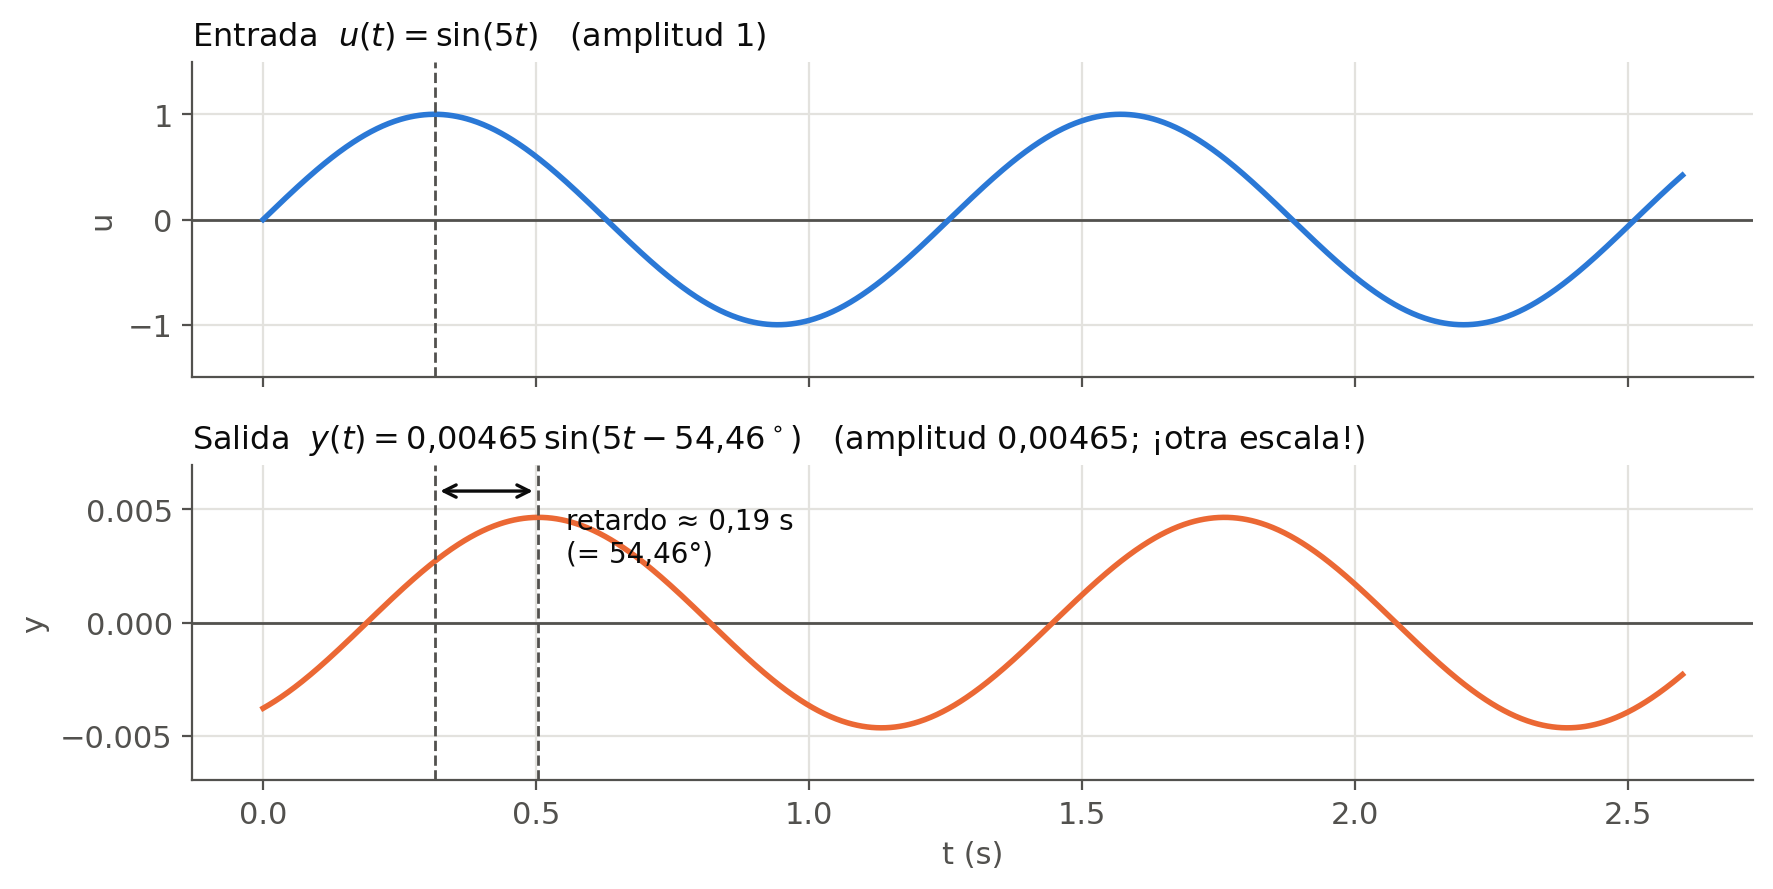
\includegraphics[height=3.0cm]{fig/senoidal_P5.png}
    \end{column}
    \begin{column}{0.54\textwidth}
      \begin{block}{Una vuelta completa}
        Una senoidal recorre $360^\circ$ en un periodo $T=2\pi/\omega$. Un retraso de $\varphi$ grados es la fracción $\varphi/360$ de ese periodo:
        \quad $\Delta t=\dfrac{\varphi}{360^\circ}\,T=\dfrac{\varphi_{\text{rad}}}{\omega}$
      \end{block}
    \end{column}
  \end{columns}

  \uncover<2->{%
  \begin{block}{Ejemplo: $\varphi=54.46^\circ$ a $\omega=5$\,rad/s (el $P(j5)$ del paso 2)}
    $T=2\pi/5=1.257$\,s \quad $\Rightarrow$ \quad $\Delta t=\dfrac{54.46}{360}\cdot1.257=\boxed{0.190\ \text{s}}$.\quad En radianes: $54.46^\circ=0.9505$\,rad y $\dfrac{0.9505}{5}=0.190$\,s.
  \end{block}}

  \uncover<3->{%
  \begin{alertblock}{Ojo: los mismos grados no son el mismo tiempo}
    La fase se mide como \emph{ángulo}. Para pasarla a segundos hay que dividir por $\omega$: $54.46^\circ$ a $\omega=50$\,rad/s son solo $0.019$\,s.
  \end{alertblock}}
\end{frame}

% ------------------------------------------------------------
\begin{frame}{Lo que tenemos y la pregunta que falta}
  \small
  \setlength{\parskip}{3pt}
  \begin{block}{Hasta ahora}
    Con $P(s)=\dfrac{1}{(s+5)(s+30)}$ calculamos un punto: \quad $P(j5)=0.00465\,\ang{-54.46}$, es decir, $-46.65$\,dB y $-54.46^\circ$.\\
    Significa: si entra una senoidal de frecuencia $\omega=5$\,rad/s, sale otra senoidal de amplitud $0.00465$ y retrasada $54.46^\circ$.
  \end{block}

  \uncover<2->{%
  \begin{alertblock}{La pregunta}
    ¿Y a $\omega=0.1$? ¿Y a $\omega=100$? Un sistema real recibe señales de \textbf{muchas frecuencias}. Hay que saber cuánto amplifica o atenúa, y cuánto retrasa, \textbf{cada una}.
  \end{alertblock}}

  \uncover<3->{%
  \begin{block}{Por qué importa en QFT}
    Los requisitos de diseño (rechazo de perturbaciones, seguimiento, márgenes) se plantean \textbf{frecuencia a frecuencia}. Más adelante, en cada $\omega$ habrá un punto (o una nube de puntos si la planta es incierta) en el Nichols chart.
  \end{block}}
\end{frame}

% ------------------------------------------------------------
\begin{frame}{La frecuencia: $\omega$ en rad/s y $f$ en Hz}
  \small
  \setlength{\parskip}{3pt}
  \begin{block}{Dos formas de medir la misma cosa}
    Una senoidal $\sin(\omega t)$ repite su forma cada $T=\dfrac{2\pi}{\omega}$ segundos. Su frecuencia en \textbf{Hz} es $f=\dfrac{1}{T}=\dfrac{\omega}{2\pi}$, es decir, $\omega=2\pi f$.\\
    $\omega$ (rad/s) es la que aparece en $s=j\omega$; $f$ (Hz) es la que usamos en la vida diaria.
  \end{block}

  \begin{center}
    \renewcommand{\arraystretch}{1.2}
    \begin{tabular}{rrr}
      \hline
      $\omega$ (rad/s) & $f$ (Hz) & Periodo $T$ (s) \\
      \hline
      1 & 0.159 & 6.283 \\
      5 & 0.796 & 1.257 \\
      10 & 1.592 & 0.628 \\
      100 & 15.92 & 0.0628 \\
      \hline
    \end{tabular}
  \end{center}

  \uncover<2->{%
  \begin{block}{Ojo}
    En este curso, salvo que se diga lo contrario, la frecuencia es $\omega$ en \textbf{rad/s}. Con $\omega=5$ el periodo es $1.257$\,s, como en la figura del paso 2.
  \end{block}}
\end{frame}

% ------------------------------------------------------------
\begin{frame}{Respuesta en frecuencia: $P(j\omega)$ como función de $\omega$}
  \small
  \setlength{\parskip}{3pt}
  \begin{block}{Definición}
    La \textbf{respuesta en frecuencia} de $P(s)$ es la función $P(j\omega)$ para todo $\omega\ge0$. Para cada $\omega$ es un número complejo (paso 1), así que tiene dos partes reales:
  \end{block}

  \begin{columns}[T]
    \begin{column}{0.48\textwidth}
      \begin{block}{Magnitud}
        $|P(j\omega)|$: cuánto se amplifica o atenúa la señal. En decibelios: $20\log_{10}|P(j\omega)|$.
      \end{block}
    \end{column}
    \begin{column}{0.48\textwidth}
      \begin{block}{Fase}
        $\angle P(j\omega)=\operatorname{atan2}(\operatorname{Im},\operatorname{Re})$: cuánto se adelanta ($+$) o se retrasa ($-$) la señal.
      \end{block}
    \end{column}
  \end{columns}

  \uncover<2->{%
  \begin{alertblock}{Cómo se calcula (receta del paso 2)}
    Para cada $\omega$: sustituir $s=j\omega$ en \textbf{toda} la función, calcular distancias y ángulos de cada factor, y combinar. Los \textbf{polos} del denominador restan magnitud y fase. Los \textbf{ceros} del numerador las suman.
  \end{alertblock}}
\end{frame}

% ------------------------------------------------------------
\begin{frame}{Un barrido a mano: $P(j\omega)$ en siete frecuencias}
  \small
  \setlength{\parskip}{3pt}
  Para $P(s)=\dfrac{1}{(s+5)(s+30)}$, calculado con la receta de antes:

  \begin{center}
    \renewcommand{\arraystretch}{1.2}
    \begin{tabular}{rrrr}
      \hline
      $\omega$ (rad/s) & $|P(j\omega)|$ & Magnitud (dB) & Fase \\
      \hline
      0.1 & $6.665\cdot10^{-3}$ & $-43.52$ & $-1.34^\circ$ \\
      1 & $6.534\cdot10^{-3}$ & $-43.70$ & $-13.22^\circ$ \\
      5 & $4.650\cdot10^{-3}$ & $-46.65$ & $-54.46^\circ$ \\
      10 & $2.828\cdot10^{-3}$ & $-50.97$ & $-81.87^\circ$ \\
      30 & $7.750\cdot10^{-4}$ & $-62.21$ & $-125.54^\circ$ \\
      100 & $9.566\cdot10^{-5}$ & $-80.39$ & $-160.44^\circ$ \\
      1000 & $9.995\cdot10^{-7}$ & $-120.00$ & $-178.00^\circ$ \\
      \hline
    \end{tabular}
  \end{center}

  \uncover<2->{%
  \begin{block}{Qué se observa}
    La magnitud cae \textbf{más de tres órdenes de magnitud} (de $6.7\cdot10^{-3}$ a $10^{-6}$) y la fase va de $0^\circ$ hacia $-180^\circ$. Las filas $\omega=5$ y $\omega=10$ ya las conoces del paso 1 y de su ejercicio.
  \end{block}}
\end{frame}

% ------------------------------------------------------------
\begin{frame}{Primer intento: dibujarlo con ejes lineales}
  \centering
  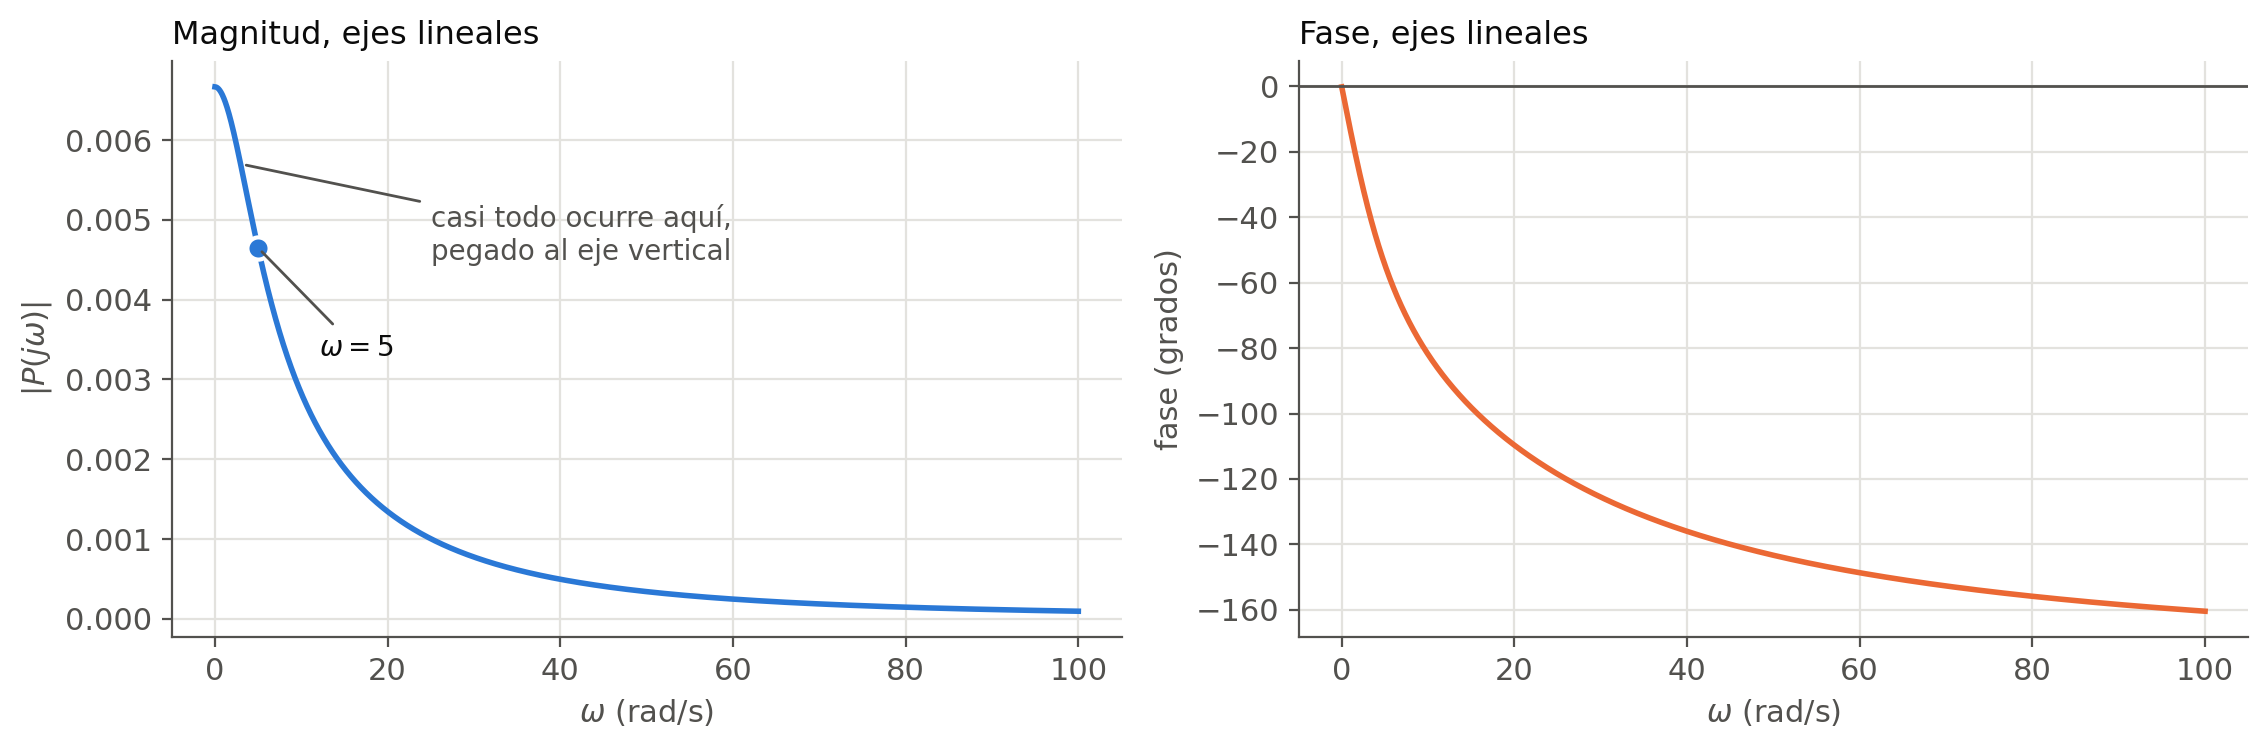
\includegraphics[width=\textwidth,height=0.6\textheight,keepaspectratio]{fig/lineal.png}

  \smallskip
  \small
  \begin{block}{Problema}
    Casi todo el cambio sucede para $\omega$ pequeña, pegado al eje vertical, y a partir de $\omega\approx40$ la magnitud parece plana en cero. Con frecuencias que abarcan \textbf{varias décadas} los ejes lineales no sirven.
  \end{block}
\end{frame}

% ------------------------------------------------------------
\begin{frame}{La solución: escala logarítmica en $\omega$ y decibelios (Bode)}
  \centering
  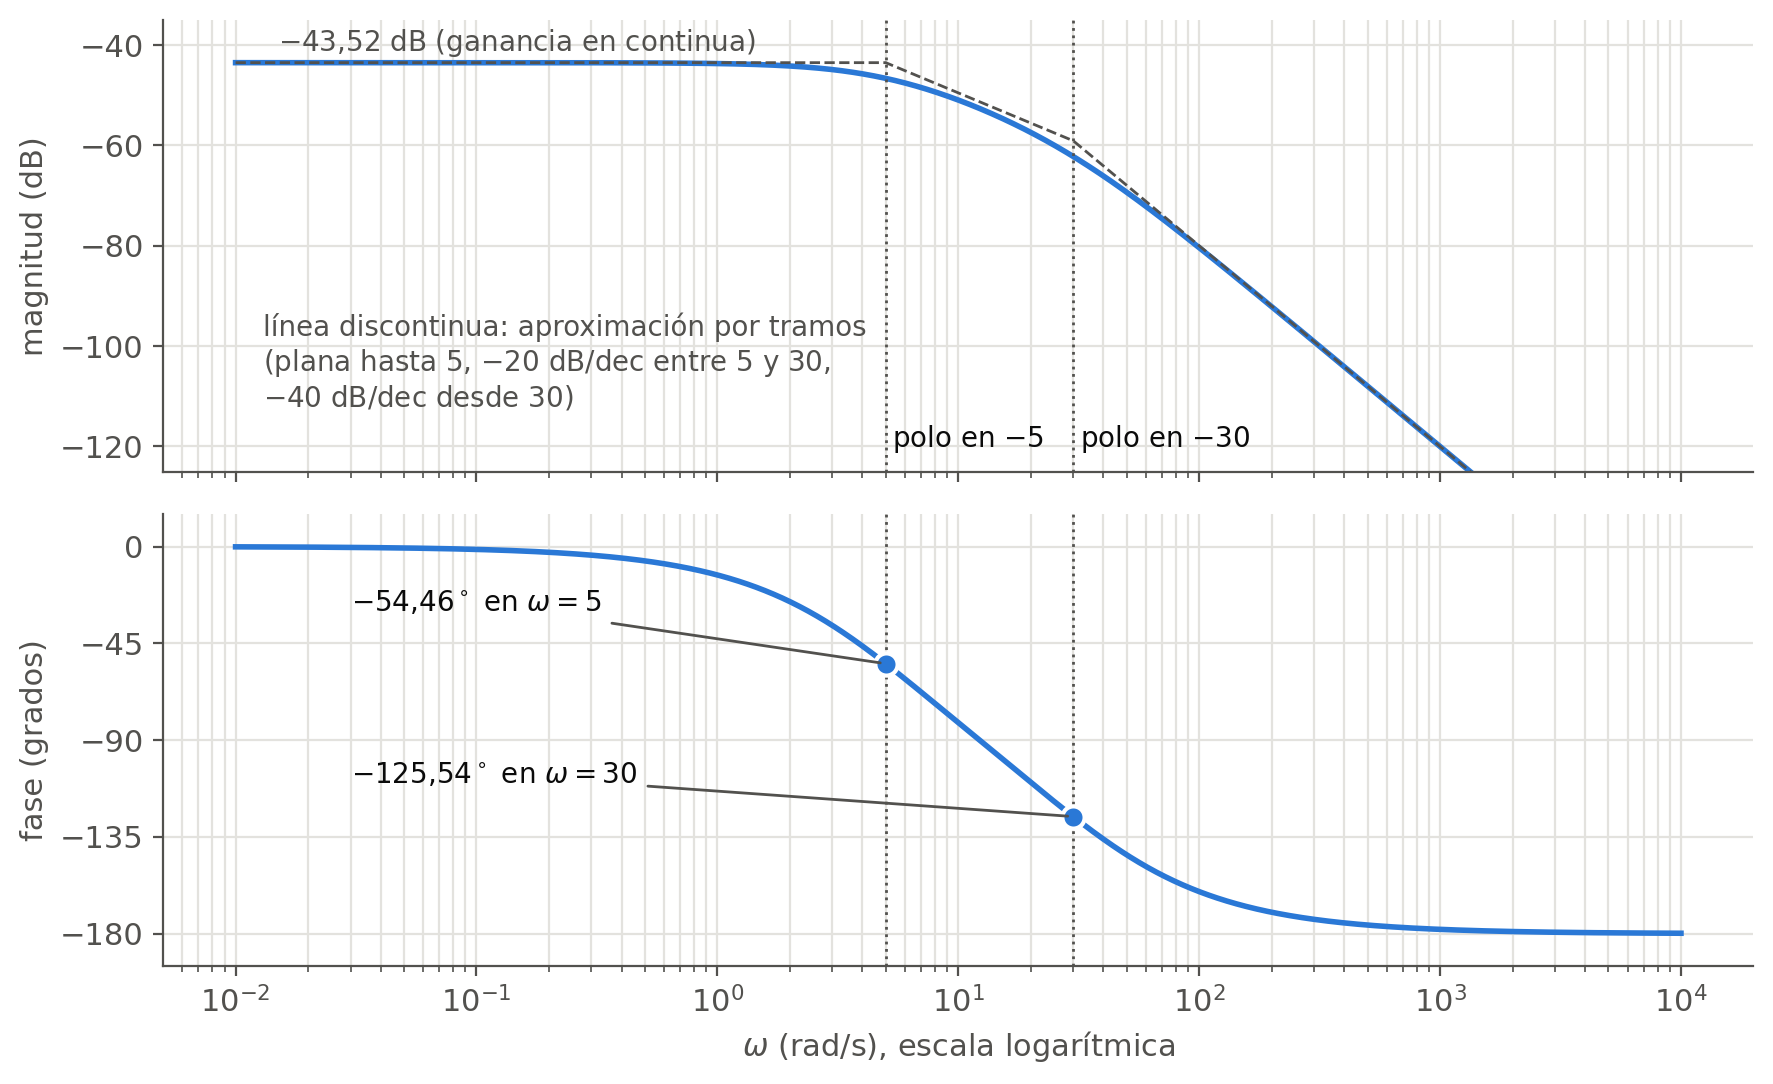
\includegraphics[width=0.9\textwidth,height=0.64\textheight,keepaspectratio]{fig/bode_P.png}

  \smallskip
  \footnotesize
  Eje horizontal: $\omega$ en escala logarítmica, donde cada \textbf{década} (factor 10) ocupa el mismo ancho. Arriba: magnitud en dB. Abajo: fase. Cada $\omega$ es un punto de cada gráfica. (Los dB y esta escala se estudian con detalle en el paso 4.)
\end{frame}

% ------------------------------------------------------------
\begin{frame}{Cómo leer la curva a partir de los polos}
  \footnotesize
  \setlength{\parskip}{2pt}
  Los polos de $P$ están en $-5$ y $-30$. Cada factor es la flecha del polo a $j\omega$ (paso 2). Según $\omega$, esa flecha se parece a algo sencillo:

  \begin{center}
    \renewcommand{\arraystretch}{1.25}
    \begin{tabular}{p{0.14\textwidth} p{0.34\textwidth} p{0.26\textwidth} p{0.14\textwidth}}
      \hline
      \textbf{Zona} & \textbf{Factores} & \textbf{Magnitud} & \textbf{Fase} \\
      \hline
      $\omega\ll5$ & $(j\omega+5)\approx5$, \ $(j\omega+30)\approx30$ & plana: $1/150$ ($-43.52$\,dB) & $\approx0^\circ$ \\
      $5\ll\omega\ll30$ & $(j\omega+5)\approx j\omega$, \ $(j\omega+30)\approx30$ & baja $20$\,dB por década & hacia $-90^\circ$ \\
      $\omega\gg30$ & ambos $\approx j\omega$ & baja $40$\,dB por década & hacia $-180^\circ$ \\
      \hline
    \end{tabular}
  \end{center}

  \uncover<2->{%
  \begin{block}{Por qué}
    Si $\omega$ es mucho menor que el polo, la flecha casi no se mueve (queda cerca de la longitud del polo y apunta casi horizontal). Si $\omega$ es mucho mayor, la flecha es casi vertical y su longitud crece como $\omega$: apunta a $90^\circ$, y como está en el denominador aporta $-90^\circ$.
  \end{block}}
\end{frame}

% ------------------------------------------------------------
\begin{frame}{El codo: qué pasa justo en $\omega=$ polo}
  \small
  \setlength{\parskip}{3pt}
  \begin{block}{Un polo en $-a$, evaluado en $\omega=a$}
    El factor es $(ja+a)=a+ja$: longitud $\sqrt2\,a$ y ángulo $45^\circ$. Como está en el denominador:\\
    \quad magnitud: $\dfrac{1}{\sqrt2\,a}$, es decir, \textbf{$3$\,dB por debajo} del valor plano $\dfrac1a$. \qquad fase: $-45^\circ$.
  \end{block}

  \uncover<2->{%
  \begin{block}{Comprobación con nuestro polo $a=5$}
    A $\omega=5$ el factor es $5+5j=7.07\,\ang{45}$. Su contribución es $20\log_{10}\dfrac{1}{7.07}=-16.99$\,dB, frente a $20\log_{10}\dfrac15=-13.98$\,dB en continua: diferencia $-3.01$\,dB. Y la fase aportada es $-45^\circ$.
  \end{block}}

  \uncover<3->{%
  \begin{alertblock}{Por eso se llama frecuencia de codo}
    Es donde la curva deja de ser plana y empieza a bajar. Cada polo real $-a$ crea un codo en $\omega=a$. En la gráfica de Bode son las líneas de puntos de $\omega=5$ y $\omega=30$.
  \end{alertblock}}
\end{frame}

% ------------------------------------------------------------
\begin{frame}{Un cero cambia la curva}
  \centering
  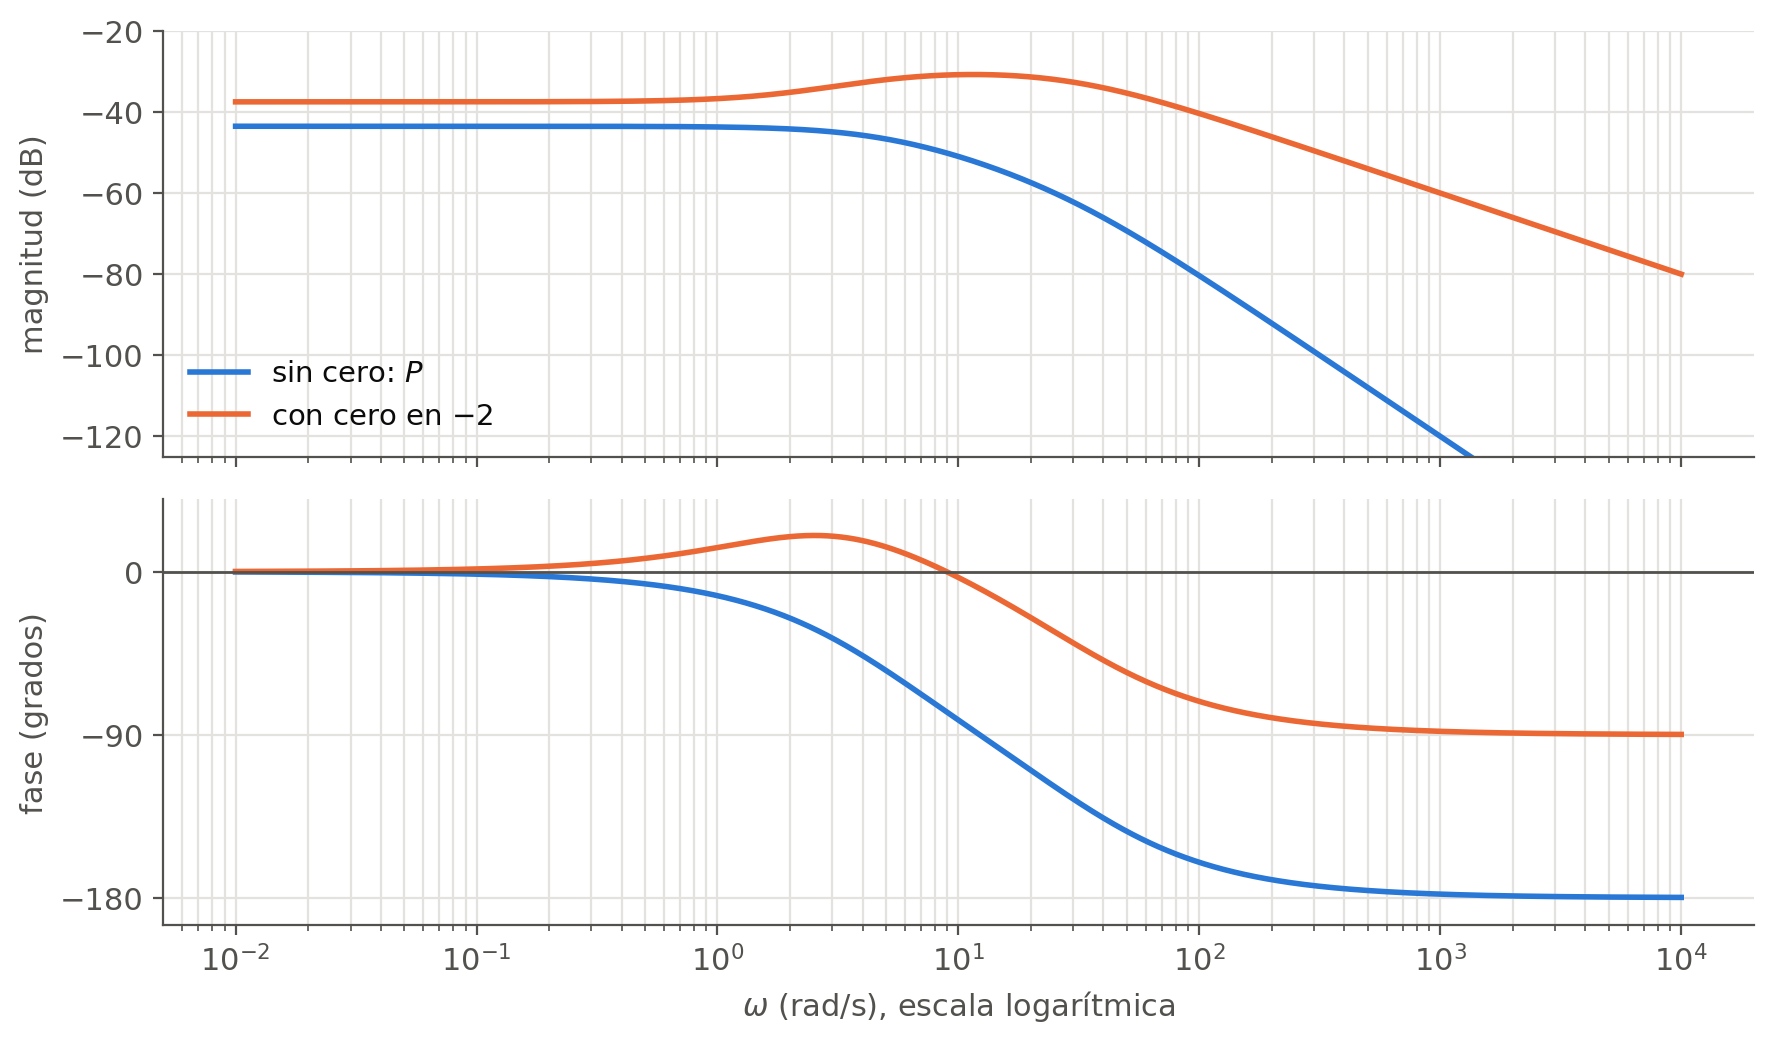
\includegraphics[width=0.85\textwidth,height=0.62\textheight,keepaspectratio]{fig/bode_cero.png}

  \smallskip
  \footnotesize
  \begin{block}{Efecto de añadir un cero en $s=-2$ (paso 2)}
    Un cero \textbf{suma} fase y magnitud: la curva baja más despacio ($-20$ en vez de $-40$\,dB/década al final) y la fase termina en $-90^\circ$ en vez de $-180^\circ$.
  \end{block}
\end{frame}

% ------------------------------------------------------------
\begin{frame}{Polos complejos: el pico}
  \centering
  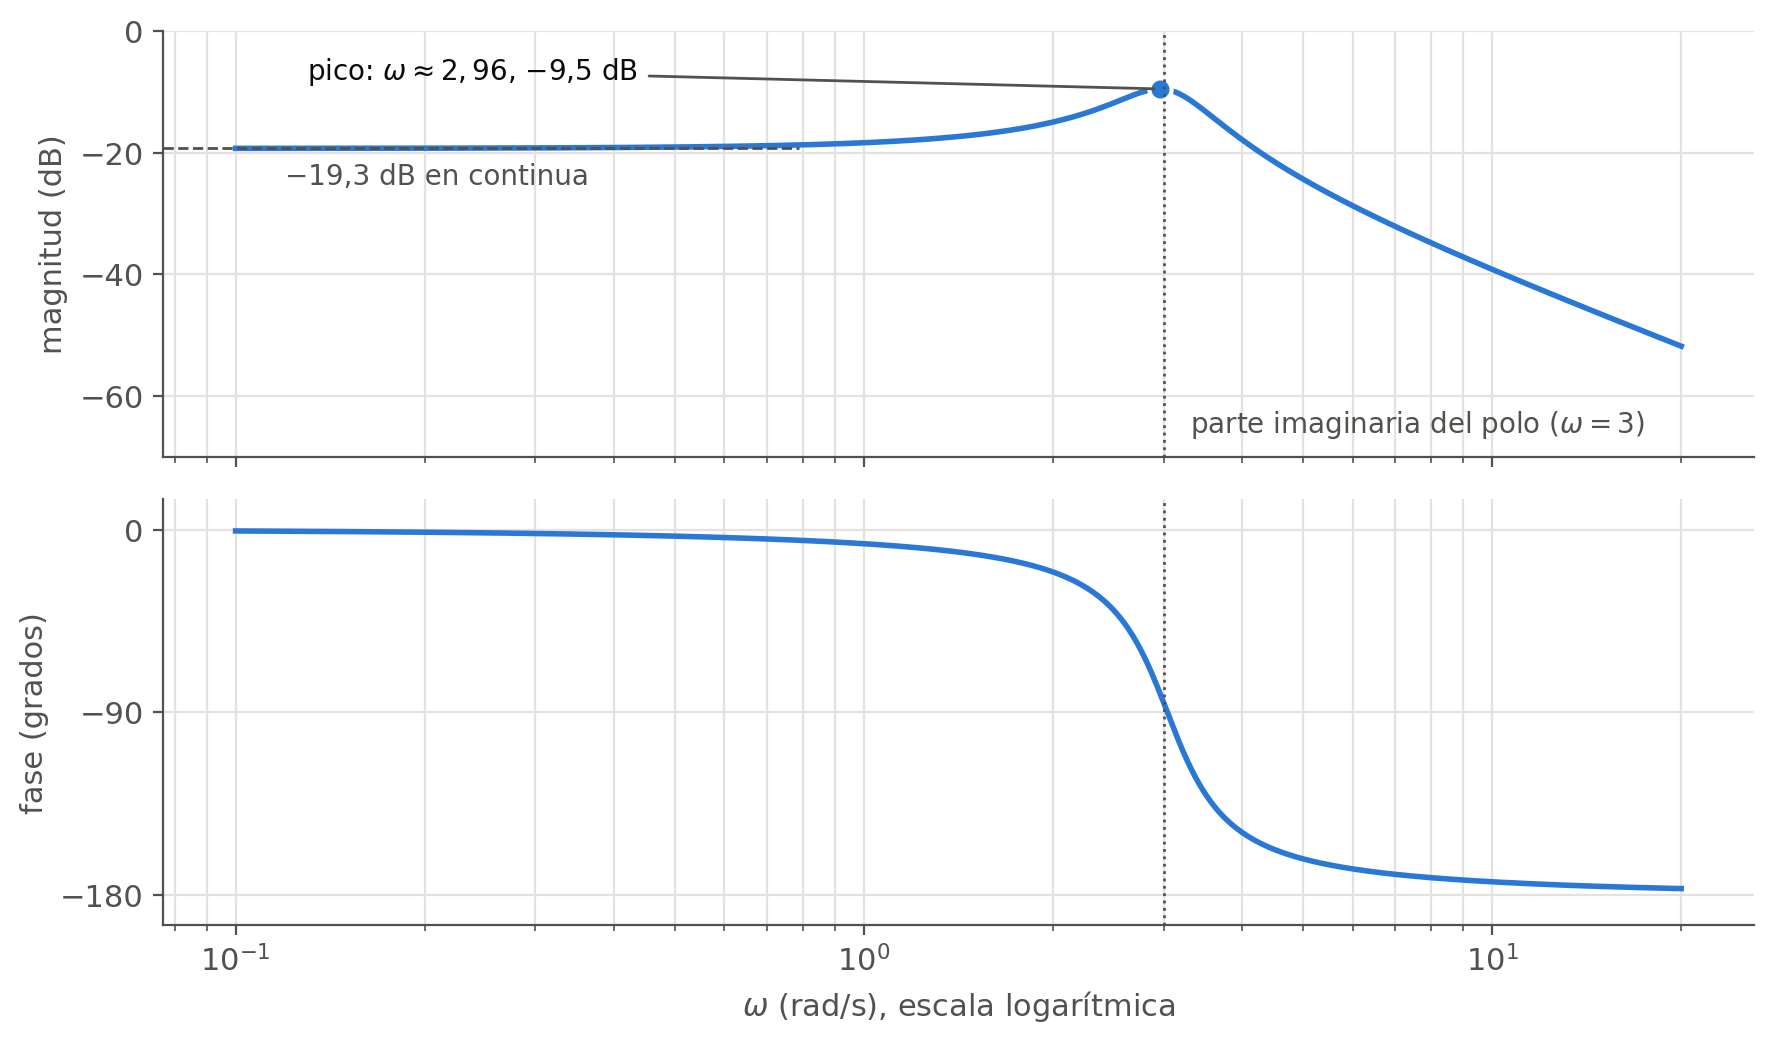
\includegraphics[width=0.9\textwidth,height=0.62\textheight,keepaspectratio]{fig/bode_resonancia.png}

  \smallskip
  \tiny
  \begin{block}{$P(s)=1/\big((s+0.5)^2+9\big)$, polos complejos $p=-0.5\pm3j$}
    \footnotesize
    En $\omega=3$, $j3$ pasa a distancia $0.5$ del polo $p$: flecha cortísima, así que $|P|$ es grande ($\approx-9.6$\,dB, frente a $-19.3$\,dB en continua). La fase cae casi $180^\circ$ de golpe.
  \end{block}
\end{frame}

% ------------------------------------------------------------
\begin{frame}{Ejercicio}
  Sea \quad $P(s)=\dfrac{20}{(s+2)(s+10)}$
  \begin{enumerate}
    \item Indica sus polos. ¿Dónde están los codos?
    \item Calcula la \textbf{ganancia en continua} $P(0)$ en dB.
    \item Calcula $P(j2)$: magnitud, dB y fase (factor a factor).
    \item ¿Hacia qué fase tiende $\angle P(j\omega)$ cuando $\omega\to\infty$? ¿Cuántos dB por década baja la magnitud al final?
  \end{enumerate}
  \vspace{4pt}
  \begin{block}{Para pensar}
    ¿Qué cambiaría si en vez de dos polos hubiera uno solo?
  \end{block}
\end{frame}

% ------------------------------------------------------------
\begin{frame}{Para programarlo: el notebook de este paso}
  \small
  Todo lo de este paso se puede \textbf{ejecutar} en el notebook \texttt{notebooks/paso03\_respuesta\_frecuencia.ipynb}.
  \begin{itemize}
    \item Python: \texttt{np.logspace}, vectorización, Bode con \texttt{semilogx}, asíntotas, el codo con \texttt{np.argmin} y el pico de resonancia.
    \item Cada cálculo a mano de las diapositivas se \textbf{comprueba} en código.
    \item Incluye celdas \emph{Tu turno} con el ejercicio del paso y la solución plegada.
  \end{itemize}
  \footnotesize Requisitos: \texttt{numpy}, \texttt{matplotlib} y, en el paso 2, \texttt{scipy}.
\end{frame}

\begin{frame}{Resumen}
  \begin{itemize}
    \item $P(j\omega)$ es un número complejo para cada frecuencia $\omega$ (rad/s, con $\omega=2\pi f$). Su conjunto es la \textbf{respuesta en frecuencia}.
    \item Magnitud $|P(j\omega)|$ (en dB: $20\log_{10}$) y fase $\angle P(j\omega)$ ($\operatorname{atan2}$).
    \item Sirve para saber cuánto amplifica y cuánto retrasa el sistema cada senoidal.
    \item Con varias décadas de $\omega$ se usan \textbf{ejes logarítmicos} (Bode).
    \item Polos reales: codo en $\omega=a$, la magnitud baja $20$\,dB/década y la fase $-90^\circ$ por polo. Ceros: lo contrario.
    \item Polos complejos: pico cerca de la parte imaginaria del polo.
  \end{itemize}
  \vspace{6pt}
  \begin{block}{Siguiente paso}
    Paso 4: decibelios y escala logarítmica en detalle (Bode), antes de la realimentación.
  \end{block}
\end{frame}

\appendix
% ------------------------------------------------------------
\begin{frame}
  \centering
  \vspace{1.2cm}
  {\Huge\bfseries Apéndice}
\end{frame}

% ------------------------------------------------------------
\begin{frame}{Solución del ejercicio: $P(s)=\dfrac{20}{(s+2)(s+10)}$}
  \footnotesize
  \setlength{\parskip}{1pt}
  \begin{block}{1. Polos y codos}
    Polos reales en $s=-2$ y $s=-10$. Codos en $\omega=2$ y $\omega=10$\,rad/s.
  \end{block}
  \begin{block}{2. Ganancia en continua}
    $P(0)=\dfrac{20}{2\cdot10}=1$, es decir, \boxed{0\ \text{dB}} (fase $0^\circ$).
  \end{block}
  \begin{block}{3. $P(j2)$ factor a factor}
    $2j+2=2.828\,\ang{45}$ \quad $2j+10=10.198\,\ang{11.31}$\\
    Magnitud: $\dfrac{20}{2.828\cdot10.198}=0.6934=\boxed{-3.18\ \text{dB}}$ \qquad Fase: $-(45^\circ+11.31^\circ)=\boxed{-56.31^\circ}$\\
  \end{block}
  \begin{block}{4. Comportamiento a frecuencias altas}
    Para $\omega\gg10$ los dos factores valen $\approx j\omega$: fase $\to-180^\circ$ y la magnitud baja $\mathbf{40}$\,dB por década.\\
    Con un solo polo: fase $\to-90^\circ$ y $20$\,dB por década.
  \end{block}
\end{frame}

\end{document}
